
\documentclass[report , a4paper, onecolumn, 12pt]{article}
\usepackage{lscape}
\usepackage{sidecap}
\usepackage{physics}
%\usepackage{bm}
\usepackage{wrapfig}
\usepackage{lipsum}
\usepackage[left=2cm,right=2cm,
    top=2cm,bottom=2cm,bindingoffset=0cm]{geometry}
\usepackage{graphicx}
\usepackage{filecontents}
\usepackage{amsmath}    
\usepackage{amsmath,amsthm,amssymb}
\usepackage{mathtext}
\usepackage[T1,T2A]{fontenc}
\usepackage[utf8]{inputenc}
\usepackage[bulgarian,english,russian]{babel}
\usepackage{braket,mleftright}
\usepackage{enumerate}
\usepackage{enumitem}
\usepackage{graphicx}
\usepackage{caption}
\captionsetup{format =plain}%
\graphicspath{{images/}{../images/}}
\usepackage{blindtext}
\usepackage{hyperref}
\usepackage{listings}
%\renewcommand{\figurename}{Рис.}
%\renewcommand{\tablename}{Табл.}
%\renewcommand*\contentsname{Оглавление}

\usepackage{hyphenat}


\title{Стационарная задача теплопроводности в балке}
\author{Василий Югов}
\date{Май 2020}
\begin{document}

\maketitle

\tableofcontents

\section{Аннотация}

В работе исследуется применение различных итерационных методов к нахождению решения уравнения Пуассона в квадрате с постоянными граничными условиями первого рода на каждой из сторон.

\section{Постановка задачи}

Исследуется классическое двумерное уравнение Пуассона

\begin{equation}
 \pdv[2]{u}{x}(x,y)+\pdv[2]{u}{y}(x,y)=0
\end{equation}

 в прямоугольнике $\Pi = [0, 1] \otimes [0, 1]$ с граничными условиями первого рода

\begin{equation}
 \label{boundary}u(0, y) = 1, \quad u(x, 1) = 2, \quad u(1, y) = 3, \quad u(x, 0) = 4
\end{equation}

Эти уравнения описывают установившееся распределение температур в бесконечно длинной однородной квадратной балке со сторонами, нагретыми до температур 1, 2, 3, 4. Коэффициент теплопроводности балки постоянен. 

Для нахождения решения уравнения Пуассона на сетке будем использовать разностную схему ``крест`` на однородной сетке:

\begin{equation}
 \frac{u_{m - 1, l} - 2 u_{m, l} + u_{m + 1, l}}{h_x^2} + \frac{u_{m,l-1} - 2 u_{m, l} + u_{m, l+1}}{h_y^2} = 0
\end{equation}


Так как задача имеет одинаковый размер вдоль двух направлений, возьмем $h_x = h_y = h = \frac{1}{N - 1}$. Тогда разностное уравнение записывается просто:

\begin{equation}
 \label{cross}u_{m, l} = \frac{1}{4}(u_{m - 1, l} + u_{m + 1, l} + u_{m,l-1} + u_{m, l+1})
\end{equation}

Граничные условия заключаются в задании $u_{m,0}$, $u_{0,l}$, $u_{m, N - 1}$, $u_{N - 1,l}$ в соответствии с \ref{boundary}.

Несложно показать, подставив в \ref{cross} разложение $u$ в ряд Тейлора в окресности узла $(m, l)$, что схема имеет второй порядок аппроксимации. В \cite{aristova} показано, что схема устойчива, т. е. система линейных уравнений \ref{cross} однозначно разрешима, и $||u_{ml}|| \le C ||f||$, где $||f||$ - норма вектора правых частей, т. е. максимум модуля значений на границе. 

Таким образом, все, что осталось - решить систему линейных уравнений \ref{cross}. Делать это будем при помощи итерационных методов: метода Якоби, метода Зейделя с шахматным упорядочением и метода верхней релаксации с шахматным упорядочением.

\section{Описание исследуемых методов}

Все исследуемые методы являются итерационными, то есть, на каждой итерации следующее приближение решения считается на основе текущего. От метода зависит лишь способ этого пересчета. Будем обозначать верхним индексом номер итерации, нижними - координаты узла.

\subsection{Критерий остановки}

Важен вопрос момента остановки вычислений. Будем пользоваться следующим критерием: на каждой итерации подсчитаем норму разницы текущего приближения и предыдыдущего $e^i = ||u^i - u^{i - 1}||$. Будем считать, что невязки аппроксимируются степенным законом: $r^i = a k^i$. Тогда можно записать

\begin{equation}
 r^i = \frac{(e^i)^2}{e^{i - 1} - e^i }
\end{equation}

Когда подсчитанная таким образом величина станет меньше ошибки, к которой мы стремимся, будем останавливать итерации.


\subsection{Исследуемые методы}

\subsubsection{Метод Якоби}

В методе Якоби используется следующая схема:

\begin{equation}
 u^{i + 1}_{ml} = \frac{1}{4} (u^{i}_{m-1, l} + u^{i}_{m, l-1} + u^{i}_{m + 1, l} + u^i_{m, l - 1}) 
\end{equation}

\subsubsection{Метод Зейделя с шахматным упорядочением}

В этом методе узлы разбиваются на две группы: с четной и нечетной суммой индексов. Для первых применяется схема как в методе Якоби:

\begin{equation}
 u^{i + 1}_{ml} = \frac{1}{4} (u^{i}_{m-1, l} + u^{i}_{m, l-1} + u^{i}_{m + 1, l} + u^i_{m, l - 1}) 
\end{equation}

Вторые считаются на основе уже найденных:

\begin{equation}
 u^{i + 1}_{ml} = \frac{1}{4} (u^{i+1}_{m-1, l} + u^{i+1}_{m, l-1} + u^{i+1}_{m + 1, l} + u^{i+1}_{m, l - 1}) 
\end{equation}

Известно, что одна итерация этого метода эквивалентна двум итерациям метода Якоби \cite{aristova}.

\subsubsection{Метод верхней релаксации с шахматным упорядочением}

Метод является модификацией предыдущего. Он характеризуется параметром $\tau\in (0,2)$, от которого зависит его эффективность. 

Узлы с четной сумой индексов рассчитываются по формуле

\begin{equation}
 u^{i + 1}_{ml} = (1-tau) u^{i}_{m,l} + \tau \frac{1}{4} (u^{i}_{m-1, l} + u^{i}_{m, l-1} + u^{i}_{m + 1, l} + u^i_{m, l - 1}) 
\end{equation}

Узлы с нечетной суммой индексов рассчитываются по формуле

\begin{equation}
 u^{i + 1}_{ml} = (1-tau) u^{i}_{m,l} + \tau \frac{1}{4} (u^{i + 1}_{m-1, l} + u^{i + 1}_{m, l-1} + u^{i + 1}_{m + 1, l} + u^{i + 1}_{m, l - 1}) 
\end{equation}

Оптимальное значение параметра $\tau$ при таком упорядочении узлов известно \cite{aristova}:

\begin{equation}
\label{tauo}\tau_o = \frac{2}{1 + \sqrt{1 - \rho^2}}
\end{equation}


Здесь $\rho$ - спектральный радиус матрицы перехода метода Якоби. Это соотношение будет в дальнейшем проверено численно.

\subsection{Теоретическое сравнение скорости сходимости}

Необходимое количество итераций для каждого метода состоит из двух множителей, первый из которых определяется необходимой точностью $ln(\varepsilon)$ \cite{aristova}. Второй множитель различается. Для метода Якоби он равен $\frac{2N^2}{\pi^2}$, для метода Зейделя $\frac{N^2}{\pi^2}$, дял метода верхней релаксации при оптимальном выборе параметра $\frac{2N}{\pi}$.

\section{Результаты}

\subsection{Численное решение}

Численное решение было успешно найдено каждым из трех методов. Использовались параметры \hbox{$N = 50, \varepsilon = 10^{-5}$}. 

Карта распределений температур в балке изображена на рис. \ref{fig:heatmap}. Одномерные графики $u(x, y)$ при фиксированных $x$ и $y$ можно увидеть на рис. \ref{fig:profiles_h} и \ref{fig:profiles_v}.

\begin{figure}[]
    \centering
    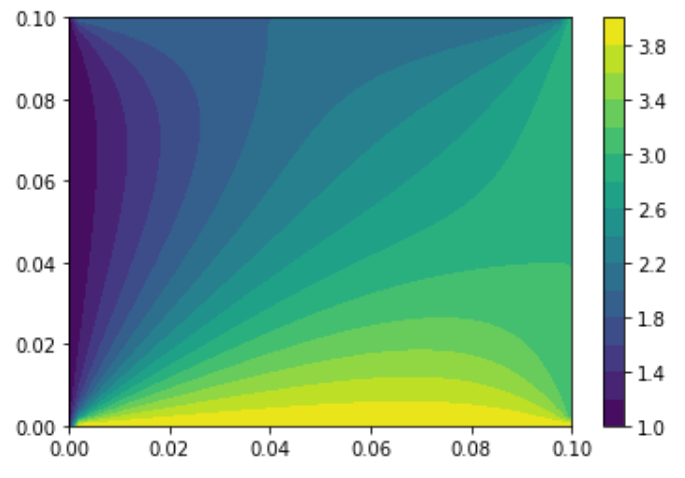
\includegraphics[width=0.6\textwidth]{heatmap}
    \caption{Карта распределения температур в балке}
    \label{fig:heatmap}
\end{figure}

\begin{figure}[]
    \centering
    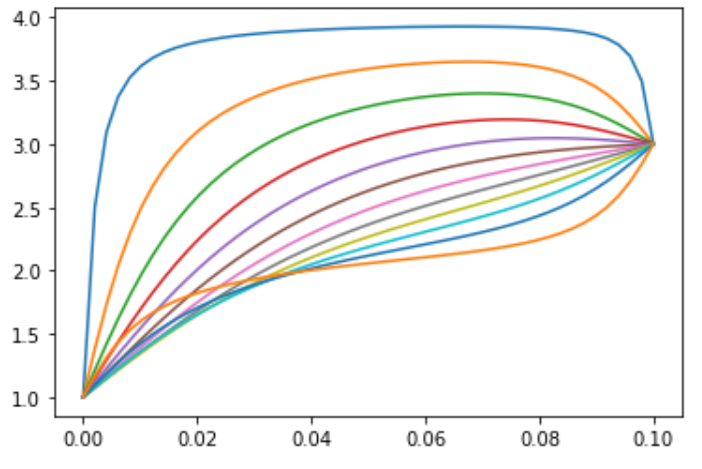
\includegraphics[width=0.6\textwidth]{profiles_h}
    \caption{Одномерные графики температур на горизонталях $y=\frac{1+4n}{49}$}
    \label{fig:profiles_h}
\end{figure}

\begin{figure}[]
    \centering
    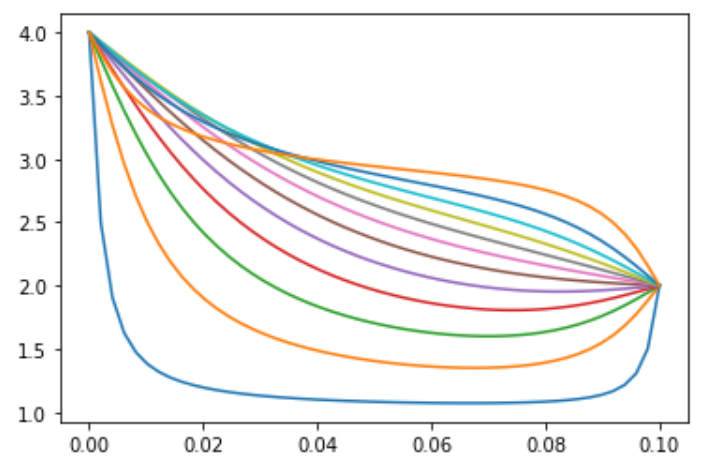
\includegraphics[width=0.6\textwidth]{profiles_v}
    \caption{Одномерные графики температур на вертикалях $x=\frac{1+4n}{49}$}
    \label{fig:profiles_v}
\end{figure}

\subsection{Численное сравнение скорости сходимости}

Для сравнения скорости сходимости методов будем использовать одинаковые параметры: $N = 50, \varepsilon = 10^{-5}$.

При таких параметрах метод Якоби потребовал $6278$ итераций, метод Зейделя - $3140$ итераций, что почти ровно в два раза меньше. Это объясняется тем, что при таком упорядочении одна итерация метода Зейделя эквивалентна двум итерациям метода Якоби. 

Метод верхней релаксации исследуем при различных значениях $\tau$ от $\tau = 1.0$ до $\tau = 2.0$ с шагом в $0.01$. Изобразим зависимость необходимого числа итераций от $\tau$ на графике(рис. \ref{fig:taus}).

\begin{figure}[]
    \centering
    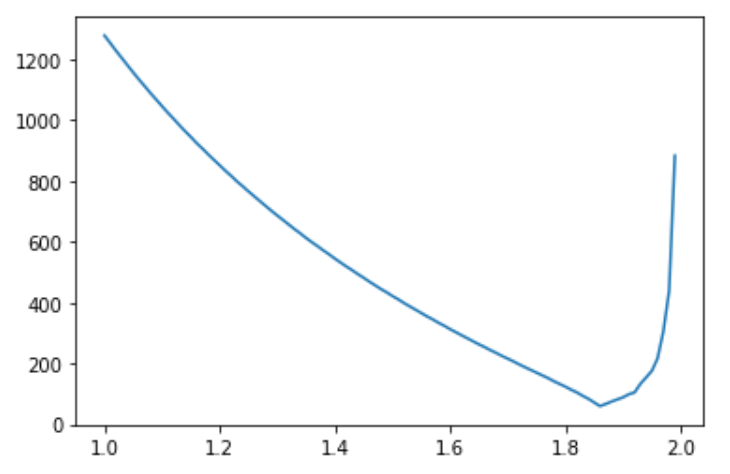
\includegraphics[width=0.6\textwidth]{taus}
    \caption{Зависимость числа итераций метода верхней релаксации от $\tau$}
    \label{fig:taus}
\end{figure}

Минимум в 60 итераций достигается при $\tau_o^e = 1.86$. 

Сравним это со значением, предсказываемым формулой \ref{tauo}. Спектральный радиус $\rho$ матрицы перехода метода Якоби найдем при помощи последовательного применения итерации метода Якоби с нулевыми граничными условиями к произвольным образом изначально заданному вектору $u$. После 10000 итераций получился результат $\rho = 0.99795$. Тогда рассчитанное по формуле \ref{tauo} оптимальное значение равно $\tau_o^t = 1.88$. Видим, что теория подтвердилась на практике.

\subsection{Скорость сходимости по сетке}

\begin{figure}[]
    \centering
    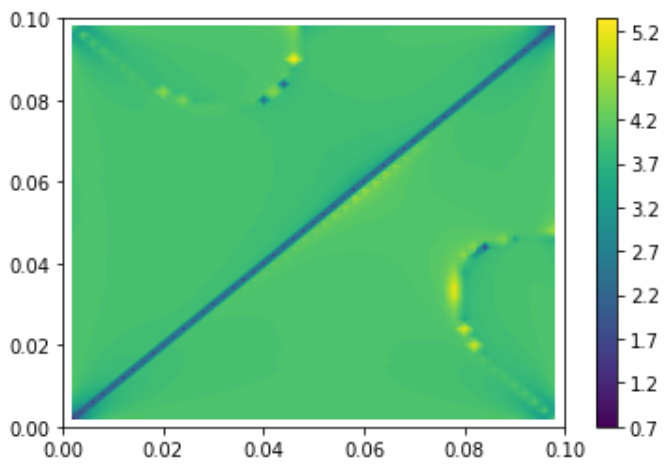
\includegraphics[width=0.6\textwidth]{errors}
    \caption{График $\frac{u^{(100)} - u^{(50)}}{u^{(200)} - u^{(100)}}$}
    \label{fig:errors}
\end{figure}

Численно оценим скорость сходимости метода ''крест`` по сетке. Для этого найдем решения $u^{(50)}, u^{(100)}, u^{(200)}$ на сетках  $N_1 = 51$, $N_2 = 101$ и $N_3 = 201$. Найдем для двух самых крупных и двух самых мелких сеток разницы в общих узлах. Встает вопрос, как сравнивать результаты. Порядок сходимости находится по формуле $2^p = \frac{||u^{(100)}-u^{(50)}||}{||u^{(200)} - u^{(100)}||}$. Найдем величину $\frac{u^{(100)} - u^{(50)}}{u^{(200)} - u^{(100)}}$ во всех общих узлах трех решеток. Она изображена на рис. \ref{fig:errors}. Из рисунка видно, что во всех точках, кроме диагонали и дуг, начинающихся в углах, это отношение равно 4, как и следует из теории. Но из-за наличия этих аномалий находить порядок сходимости на этих сетках по $L_\infty$ норме невозможно. Но можно найти его по $L_1$ норме. На общих узлах трех сеток

\begin{equation}
 ||u^{(100)} - u^{(50)}||_1 = 0.603, \quad  ||u^{(200)} - u^{(100)}||_1 = 0.161, \quad p^{(e)}=\log_2\left(\frac{||u^{(100)}-u^{(50)}||}{||u^{(200)} - u^{(100)}||}\right)=1.91
\end{equation}

Найденный порядок сходимости близок к теоретиески известному $p^{(t)} = 2$.

\section{Вывод}

Таким образом, был проведен анализ схемы ''крест`` аппроксимации уравнения Пуассона и трех итерационных методов решения полученной системы уравнений: метода Якоби, метода Зейделя с шахматной расстановкой, и метода верхней релаксации с шахматной расстановкой. Было проведено сравнение скорости работы этих методов. Также был экспериментально найден порядок сходимости схемы ''крест". 

\begin{thebibliography}{9}
\bibitem{aristova} 
Е. Н. Аристова, А. И. Лобанов
\textit{Практические занятия по вычислительной математике в МФТИ. Часть 2.}. 
МФТИ, Москва, 2015

\end{thebibliography}

\end{document}
